\newcommand{\duedate}{17 September 2026}
\documentclass{16384_doc}
\usepackage{enumitem}
\usepackage{tikz}
\usetikzlibrary{positioning,arrows,arrows.meta,matrix,fit,backgrounds,calc,math,patterns,patterns.meta,intersections,fpu}
\newcommand{\assignmentname}{Assignment 5: Lagrangian Dynamics}

\begin{document}
\maketitle

\tableofcontents

\section{Code Questions}

\begin{questions}
    \titledquestion{Double Pendulum Simulation}[40]
    In this question you will simulate the double pendulum using the equations of motion you derived previously. All the code is in the \verb!code/! folder; \verb!code/README.md! explains how to run each script. You edit and submit only \verb!double_pendulum.py!.

    Use the same conventions as your derivation: $q = [\theta_1, \theta_2]^\top$ with both angles measured from the downward vertical (counterclockwise positive), $\theta_2$ the absolute angle of link 2 rather than its angle relative to link 1, and point masses $m_1, m_2$ on massless links $\ell_1, \ell_2$. There is no applied torque in the code ($\tau = 0$). In your code, use the constants \verb!M1!, \verb!M2!, \verb!L1!, \verb!L2! and \verb!G! at the top of \verb!double_pendulum.py! rather than writing the numbers in directly, because the autograder changes them.

    \begin{enumerate}[label=\alph*.]
        \item \text{[20 points]} Implement \verb!dynamics(q, qd)!, which returns the joint accelerations $\ddot q$ as an array of shape $(2,)$. Your Euler-Lagrange equations are linear in $\ddot q$, so write them as $M(q)\ddot q = b(q, \dot q)$ and solve for $\ddot q$ with \verb!np.linalg.solve!.

        \item \text{[15 points]} Implement \verb!simulate(q0, qd0, T, dt)!. We recommend using a library like \verb!scipy.integrate.solve_ivp! to integrate the equations of motion with the supplied \verb|RTOL| and \verb|ATOL| tolerances, but also encourage you to try implementing your own integrator to learn a little about numerical integration. You'll see the difference in (c)'s energy check.

        The output format should be a tuple \verb!(t, q, qd)! of numpy arrays, sampled every \verb!dt! seconds from $0$ to $T$ inclusive (use \verb!np.arange(0, T + dt / 2, dt)!, so there are $N = T/\Delta t + 1$ samples):
        \begin{itemize}
            \item \verb!t!: the sample times $0, \Delta t, 2\Delta t, \dots, T$, shape $(N,)$.
            \item \verb!q!: the joint angles $[\theta_1, \theta_2]$ at each sample time, shape $(N, 2)$.
            \item \verb!qd!: the joint velocities $[\dot\theta_1, \dot\theta_2]$ at each sample time, shape $(N, 2)$.
        \end{itemize}
        The first row of \verb!q! and \verb!qd! is the initial state \verb!q0!, \verb!qd0!.

        Run \verb!python local_autograder.py! to check parts (a) and (b), then watch your pendulum with \verb!python visualize.py!.

        \item \text{[5 points]} With no friction and no applied torque, the total energy $E = T + V$ of the double pendulum stays constant. That gives you a way to check a simulation without knowing the right answer: if $E$ changes over time, the simulation is not exactly following the physics.

        Implement \verb!total_energy(q, qd)! in \verb!double_pendulum.py! using your $T$ and $V$ from your derivation; the autograder checks it.  Then run \verb!python energy_check.py!, which simulates the pendulum for 20 seconds and plots its total energy over time.  With \verb!solve_ivp! at the supplied tolerances the line should be flat; if you wrote your own integrator, see how far it drifts.

        \textbf{Try it (not graded).}  Run \verb!python visualize.py --chaos 5 --plot!, which simulates five pendulums whose starting $\theta_2$ values differ by only $0.001$ rad, and watch how long they stay together.  Then try a small initial angle, \verb!python visualize.py --chaos 5 --q0 10 5!, and compare.
    \end{enumerate}
\end{questions}

\section{Hands-on Lab: Drawing with the xArm7}

% STAFF TODO (not for students):
% - Set MARKER_LENGTH in lab/drawing_arm.py to the flange-to-tip length of the
%   station's marker holder. A centimetre or two off is fine (calibration
%   cancels it, see the planar-arm subsection), but it should be roughly right.
%   It must be under ~16 cm: in the home pose the flange is 17 cm above the table.
% - The holder must let the marker slide back at least PRESS (1 mm); a rigid
%   mount pushes the tip into the table.
% - Tape a US-letter sheet, landscape, on the table in front of each arm,
%   centred 50 cm straight out from the base (its edges 39 and 61 cm out). From
%   there every corner can be reached both from the home pose and in the drawing
%   pose; the simulator's sheet sits in the same place.

In this section the xArm7 holds a marker and writes on a sheet of paper.  You
already have most of the pieces: your Assignment~4 \verb!Robot! does the
inverse kinematics, and the arm is driven exactly as you drove planar chains
there.  What is new is where the paper is.  You will find it the way a
technician would: touch the marker to its four corners, and turn those four
points into a coordinate frame for the sheet.  Then you will draw the letters
\textbf{RKD} on screen, run them in simulation, and finally watch the real arm
write them.

\subsection{The xArm7 as a Planar Arm}

Hold joints 3 and 5 at zero and every joint of the xArm7 lies in one vertical
plane, the one joint 1 turns.  Joints 2, 4 and 6 are then three parallel hinges
in that plane: a planar RRR arm standing up, with the marker on the end of its
third link.  To put the marker tip on a point $\vec{p} = [p_x, p_y, p_z]^\top$ in
the robot's base frame,
\begin{enumerate}
    \item joint 1 turns to face it, $q_1 = \operatorname{atan2}(p_y, p_x)$;
    \item in that plane, $\vec{p}$ is at $r = \sqrt{p_x^2 + p_y^2}$ out and
          $z = p_z - 0.267$ m up from the shoulder;
    \item your \verb!Robot.inverse_kinematics! solves the RRR for the goal
          $[r, z, \phi]$, where $\phi$ is the angle of the third link that keeps
          the marker pointing into the paper.
\end{enumerate}
\verb!lab/drawing_arm.py! does steps 1 and 2 and calls your IK for step 3.  It
measures the three link lengths and the joint offsets from UFACTORY's own model
of the arm, so you don't have to.  Your IK takes 100 steps of size $0.1$, which
was sized for the metre-long links of Assignment 4.  The xArm's links are about
a third of that, so one call only gets part of the way, and \verb!drawing_arm.py!
calls it again from its own answer until the marker lands within 1~mm.

The marker always points straight down, and joint 7 turns against joint 1 so
that the tool never rotates about the vertical either.  The tool only ever
translates: in calibration and in drawing alike, it keeps one fixed
orientation.  That is what makes the drawing independent of the marker.  The
code computes the tip as $\vec{t} = \vec{f} + \mat{R}\,[0, 0, \ell]^\top$ from the
flange position $\vec{f}$ and orientation $\mat{R}$, with $\ell$ the nominal
\verb!MARKER_LENGTH!; the real tip is $\vec{f} + \mat{R}\,\vec{d}$ for some
$\vec{d}$ nobody measured.  With $\mat{R}$ fixed, the two differ by the same
vector everywhere, so the calibration, made with the computed tip, finds the
paper shifted by that vector, and the drawing, planned with the computed tip,
puts the real tip back on it.  (The simulator's marker is 18~mm longer and 5~mm
off-axis compared with \verb!MARKER_LENGTH!, and the ink still lands within
about a millimetre.)  It is also why you never push the marker onto the paper
by hand: a hand would hold it at a different angle each time.

\subsection{Setting Up}

The lab uses the course robot library, \verb!xarm7_lib!, the same one as the
Assignment 3 lab.  Update it before you start:
\begin{verbatim}
    git clone https://github.com/CMU-16384-2026-Fall/16384-robot-lib
    cd 16384-robot-lib
    git pull                        # if you already had it cloned
    conda env update -f environment.yml
    conda activate 16384
\end{verbatim}
Run every command in this section from the \verb!lab! folder.  As before, the
same scripts drive the real arm when the \verb!ROBOT_IP! environment variable is
set, and a MuJoCo simulation, shown in your browser, when it is not.  Everything
up to the last part can be done at home.

\begin{figure}[h]
\centering
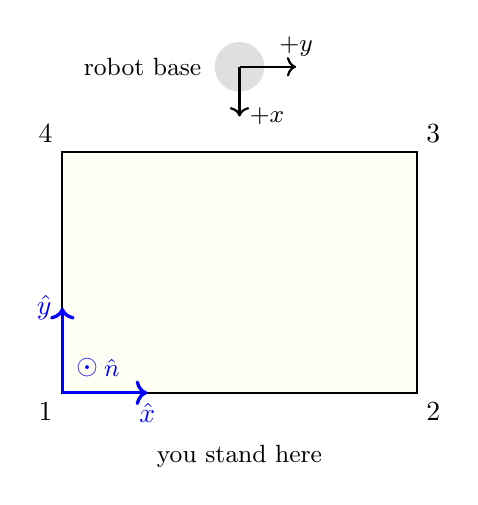
\begin{tikzpicture}[scale=0.9]
    \fill[gray!25] (2.5,4.6) circle (0.35);
    \node[left] at (2.1,4.6) {\small robot base};
    \draw[->, thick] (2.5,4.6) -- (2.5,3.9) node[right] {\small $+x$};
    \draw[->, thick] (2.5,4.6) -- (3.3,4.6) node[above] {\small $+y$};
    \draw[thick, fill=yellow!4] (0,0) rectangle (5,3.4);
    \node[below left] at (0,0) {1};
    \node[below right] at (5,0) {2};
    \node[above right] at (5,3.4) {3};
    \node[above left] at (0,3.4) {4};
    \draw[->, very thick, blue] (0,0) -- (1.2,0) node[below] {$\hat{x}$};
    \draw[->, very thick, blue] (0,0) -- (0,1.2) node[left] {$\hat{y}$};
    \node[blue] at (0.35,0.35) {$\odot$};
    \node[blue, right] at (0.45,0.35) {\small $\hat{n}$};
    \node at (2.5,-0.9) {\small you stand here};
\end{tikzpicture}
\caption{The sheet from above.  You touch corners 1--4 in order; the paper
frame has its origin at corner 1, $\hat{x}$ towards corner 2, and $\hat{n}$ out of
the paper.}
\label{fig:paper}
\end{figure}

\begin{questions}
    \setcounter{question}{1}
    \titledquestion{Drawing RKD on the xArm7}[50]

    This question is graded on your \verb!plane.py! (autograded) and on one
    video of the real arm.  There is nothing to write up.

    \begin{enumerate}[label=\alph*.]
        \item \text{[10 points]} \textbf{The paper's frame.}  Calibration gives
        you four touched corners $\vec{p}_1, \vec{p}_2, \vec{p}_3, \vec{p}_4$ in
        the robot's base frame, in the order of Figure~\ref{fig:paper}.  They
        will not lie exactly on one plane: the paper isn't perfectly flat, and
        each touch is only as good as your eye.  So the frame uses all four:
        \begin{itemize}
            \item the unit normal from the cross product of the diagonals,
                  $\hat{n} = \vec{n} / \|\vec{n}\|$ with
                  $\vec{n} = (\vec{p}_3 - \vec{p}_1) \times (\vec{p}_4 - \vec{p}_2)$;
                  it is perpendicular to both diagonals, weighs all four touches
                  alike, and with the corners in this order points up out of the
                  paper;
            \item the plane through the centroid
                  $\vec{c} = \frac{1}{4}\sum_i \vec{p}_i$;
            \item the origin $\vec{o}$: corner 1, moved along $\hat{n}$ onto that
                  plane;
            \item the $x$ axis $\hat{x}$: $\vec{p}_2 - \vec{p}_1$ with its
                  component along $\hat{n}$ removed, normalized; and
                  $\hat{y} = \hat{n} \times \hat{x}$.
        \end{itemize}
        Work out the formulas for $\vec{o}$ and $\hat{x}$, and implement them in
        \verb!lab/plane.py!: \verb!plane_frame! returns the $4 \times 4$
        homogeneous transform
        \[
            \mat{H} = \begin{bmatrix} \hat{x} & \hat{y} & \hat{n} & \vec{o} \\
                                      0 & 0 & 0 & 1 \end{bmatrix};
        \]
        \verb!paper_to_robot! maps a point $(u, v)$ on the paper, at height $h$
        above it, to $\mat{H}\,[u, v, h, 1]^\top$; and \verb!robot_to_paper! is its
        inverse, written without a matrix inverse.  These three are autograded,
        on randomly perturbed corners as in Question~1.  Then check them before
        going anywhere near the arm:
        \begin{verbatim}
python check_plane.py
\end{verbatim}
        It tries your frame on sheets whose answer is known (flat, turned,
        tilted, a whiteboard standing up), on noisy touches checked against
        every property the formula promises, and on the graded cases, the same
        ones \verb!local_autograder.py -p plane! runs from \verb!code/!.  Every
        failure says what is wrong.  A wrong frame sends the marker
        into the table, so do not take the lab past this point until it reports
        no failures.

        \item \textbf{Draw it, in simulation} (not graded, but do it before your
        lab session).
        \begin{enumerate}[label=(\roman*)]
            \item Copy your Assignment 4 \verb!robot.py! over
                  \verb!lab/robot.py!, whole and unchanged, for example
                  \verb!cp ../../Assignment4/ex2/robot.py robot.py! (the
                  \verb!robot.py! in \verb!ex1!, \verb!ex2! and \verb!ex3! is the
                  same class; take the one with your IK in it).  The forward
                  kinematics, Jacobian and gradient-descent IK you already wrote
                  are what the arm runs.  If it is still the stub, or the IK isn't
                  filled in, the lab scripts say so before anything moves.
            \item Calibrate the simulator's sheet: \verb!python calibrate.py!.
                  The simulator has a sheet of paper of its own, placed a little
                  crooked on purpose.  It touches the four corners with your IK,
                  builds the frame with your \verb!plane.py!, and tells you how far
                  your frame is from the sheet's true one.  It should be within a
                  couple of millimetres.  Then practise the real arm's procedure:
                  \verb!python calibrate.py --manual! has you jog the marker onto
                  each corner yourself, with the keys of part (c), while it tells
                  you how far the tip is from the paper.
            \item Draw the strokes for the letters \textbf{RKD}:
                  \verb!python sketch.py strokes/rkd.json!.  Left-click to place
                  points, right-click to finish a stroke; the window lists the
                  other keys.  Each stroke is traced without lifting the marker,
                  so think about where to put the breaks.  Closing the window
                  saves the file.  The strokes are stored in metres on the sheet,
                  from corner 1, so the same file draws in simulation and on the
                  real arm.
            \item Run it: \verb!python draw.py strokes/rkd.json!.  Your IK is
                  solved along the whole path first, which takes a few seconds,
                  and any point it can't reach stops the run before anything
                  moves.  Then the simulated arm writes on its sheet, and ink
                  appears where the marker meets the paper.  The result is saved
                  as \verb!results/rkd-sim.png!: your strokes, dashed, beside the
                  path the marker really took.
        \end{enumerate}

        \item \text{[40 points]} \textbf{Draw it on the xArm7.}  Graded by hand,
        from your video.  The sheet is taped to the table for
        you, about 50~cm straight out from the base; don't move it.  In lab, with
        \verb!ROBOT_IP! set:
        \begin{enumerate}[label=(\roman*)]
            \item \verb!git pull! your code onto the lab machine, and run
                  \verb!python check_plane.py! once more.
            \item \verb!python calibrate.py!.
                  \begin{itemize}
                      \item The arm moves to the home pose of the Assignment 3 lab:
                            marker pointing down, a few centimetres over the table,
                            with joints 1, 4 and 7 turning about vertical axes.  For
                            each corner in turn, swing the arm by hand until the
                            marker is over the corner, and press enter.  It only
                            has to be close: if the arm won't go all the way, press
                            enter where it stops, and the jog below covers the
                            rest.  Only those three joints are free.  If
                            you push one of the others out of place, or take the
                            marker out of the area the arm can draw on, the arm
                            locks where it is, asks you to let go, and moves back.
                      \item The arm moves to its drawing pose, marker down, above
                            corner 1.  (It raises its shoulder on the way: a
                            straight move between the two poses would take the
                            marker through the table.)
                      \item For each corner, jog the marker until the tip just
                            touches it: \verb!w!/\verb!s! move it away from you and
                            towards you, \verb!a!/\verb!d! left and right,
                            \verb!r!/\verb!f! up and down, and \verb!1!, \verb!2!,
                            \verb!3! set the step to 0.5, 2 or 10~mm.  Come down the
                            last few millimetres in 0.5~mm steps, and press enter
                            when the tip touches.
                  \end{itemize}
            \item \verb!python draw.py strokes/rkd.json --plan-only! plans the
                  drawing on your real sheet without moving anything.  Look at
                  \verb!results/rkd-plan.png!.
            \item \verb!python draw.py strokes/rkd.json!, hand on the e-stop.
        \end{enumerate}

        \begin{tcolorbox}[colback=red!5, colframe=red!60!black,
            title={Safety: Read this before you touch the robot}]
        \begin{itemize}
          \item \textbf{The e-stop.} Know where it is before you start, and keep
                a hand on it while the arm draws.  Press it for anything you did
                not expect.  Stopping the arm costs you nothing.
          \item \textbf{Stay out of the workspace} while the arm moves under its
                own power.  The only time you touch it is during calibration, when
                the script says the arm is free.
          \item \textbf{``Press enter when your hands are clear'' means it.}
                Every move the scripts make on their own waits for that prompt.
          \item \textbf{The safety box} is the one from Assignment 3:
                $x \in [-0.10, 0.70]$, $y \in [-0.45, 0.45]$, $z \in [0, 0.80]$ m.
                \verb!draw.py! checks the whole drawing against it, and against
                self-collision, before anything moves.  It does \emph{not} know
                about the marker, so the marker is yours to keep off the table:
                that is what the calibration is for.
          \item \textbf{If the marker digs in}, press the e-stop.  The drawing
                presses 1 mm below the surface you touched, which a sprung marker
                holder absorbs.  More than that means the calibration is off:
                calibrate again.
        \end{itemize}
        \end{tcolorbox}

        \textbf{Deliverable.}  One video, a phone is fine, showing the arm write
        RKD from start to finish, with the paper visible.  Put it in
        \verb!lab/handin/!.  \verb!create_submission.py! packages it with your
        \verb!lab/robot.py!, \verb!lab/plane.py!, your strokes, your
        calibrations and \verb!lab/results!.
    \end{enumerate}
\end{questions}

\begin{submissionChecklist}
        \item Run \verb!local_autograder.py! and \verb!lab/check_plane.py!, and confirm they report no failures.
        \item Put your drawing video in \verb!lab/handin!.
        \item Run \verb!python create_submission.py! from the \verb!code! folder.
        \item Rename \verb|submission.zip| and upload \verb!<andrew_id>.zip! to Gradescope.  There is no PDF to submit.
        \item The code is autograded, with no limit on number of submissions within the mandated deadline.
\end{submissionChecklist}

\end{document}
